

Este sistema consta de $n$ pistones hidráulicos ubicados espacialmente de manera que cada uno sostenga un eje del vehículo que se desea elevar. En este análisis sólo nos vamos a concentrar en la altura de pistón respecto a un nivel de referencia que sería cero. En este caso específico se considerarán seis actuadores  los cuales tienen una distribución de un arreglo 2x3.

%\begin{figure}[!t]
%\centering
%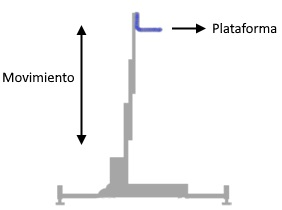
\includegraphics[width=2in]{imagenes/plataforma.jpg}
%\caption{Módulo elevador}
%\label{fig_plataforma}
%\end{figure}

\subsection{Pistón hidráulico}
Para simular el comportamiento de este actuador se consideró el modelo propuesto en \cite{Electro-hydraulic_actuator}. La planta es definida por un sistema no lineal, esta incluye un modelo de fricción, de una servo válvula y la dinámica de un cilindro externo que representa la carga. El esquema de la Figura \ref{fig_esquemapiston} describe físicamente el actuador considerado. Cada pistón cuenta con una cámara dividida por un émbolo, se bombea fluido desde $u_2$, por simplicidad consideraremos este flujo constante. La electro válvula $u$ controla el flujo para cada una de las cámaras $A$ y $B$, la diferencia de presión entre estas y el peso de la carga definirá el movimiento y la posición del pistón. 

\begin{figure}[!t]
	\centering
	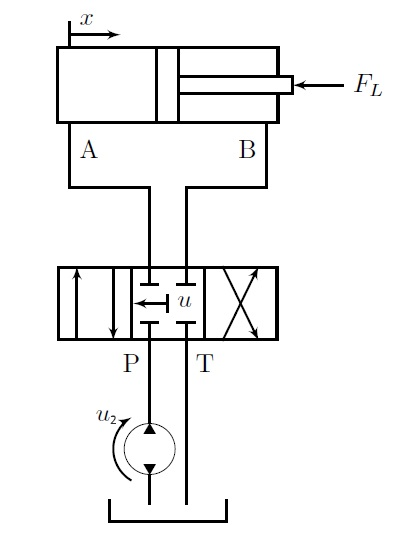
\includegraphics[width=2.3in]{imagenes/esquemapiston.jpg}
	\caption{Esquema físico}
	\label{fig_esquemapiston}
\end{figure}

En este trabajo se diseñó un control robusto para llevar el error de posición a cero asumiendo que el vector de estados es completamente medible. Las ecuaciones de estado que resultan son las mostradas en \ref{eq_statespace}, dónde $x_1$ y $x_2$ son la posición y velocidad del pistón respectivamente, $x_3$ es la presión de la carga, $x_4$ y $x_5$ son la dinámica y el control de la servo válvula.

\begin{eqnarray}
\label{eq_statespace}
\dot{x}_1&=&x_2\\
\nonumber \dot{x}_2&=&\frac{1}{m}(-k_sx_1-b_dx_2+\Lambda_ax_3-Fr-M)\\ 
\nonumber \dot{x}_3&=&-\alpha x_2-\beta x_3+(\gamma \sqrt{Ps-sgn(x_4)x_3})x_4\\
\nonumber \dot{x}_4&=&x_5\\
\nonumber \dot{x}_5&=&-c_nx_4-b_nx_5+a_nu
\end{eqnarray}

Los valores de los parámeros del modelo usados para simulación son presentados en la Tabla \ref{tab_valoresmodelo}. Con estos valores la respuesta del pistón es estable. Adicionalmente el sistema se configuró en lazo cerrado  y se agregó un control proporcional e integral, con el fin de que el sistema tenga error cero al estabilizarse y coincida con el valor de referencia que será el correspondiente al consensus.









